\chapter{Processi software}
\begin{redbar}
Un \textbf{processo software} è un insieme di attività correlate che porta alla produzione di un sistema software.    
\end{redbar}

Come già discusso, esistono diversi tipi di sistemi software e non esiste un metodo di ingegneria del software universale applicabile a tutti. Nonostante l'esistenza di molti processi software diversi, tutti devono includere, in qualche forma, le seguenti quattro attività fondamentali dell'ingegneria del software:
\begin{enumerate}
    \item \textit{Specificazione del software:} Definire la funzionalità del software e le limitazioni operative.
    \item \textit{Sviluppo del software:} Produrre il software in base alla specifica.
    \item \textit{Validazione del software:} Validare il software per garantire che soddisfi le esigenze del cliente.
    \item \textit{Evoluzione del software:} Evolvere il software per soddisfare i bisogni in continua evoluzione del cliente.
\end{enumerate}
Quando descriviamo i processi, parliamo solitamente delle attività, dell'ordine in cui vengono eseguite e del ruolo delle persone coinvolte, dei prodotti generati e delle condizioni che influenzano l'esecuzione delle attività:
\begin{enumerate}
    \item \textit{Prodotti o deliverable:} Sono i risultati di un'attività di processo.
    \item \textit{Ruoli:} Rappresentano le responsabilità delle persone coinvolte nel processo.
    \item \textit{Precondizioni e postcondizioni:} Condizioni che devono essere verificate prima e dopo    l'esecuzione di un'attività di processo o la produzione di un prodotto.
\end{enumerate}
Nei processi "plan-driven", tutte le attività di processo sono pianificate in anticipo e i progressi vengono misurati rispetto a questo piano. Nei processi agili, la pianificazione è incrementale e continua durante lo sviluppo del software, rendendo più facile adattare il processo a nuovi requisiti. Ogni approccio è adatto a diversi tipi di software; in generale, per grandi sistemi è necessario trovare un equilibrio tra processi pianificati e agili.

\section{Modelli di processo software}
Un modello di processo software (chiamato a volte Ciclo di Vita del Software o SDLC) è una rappresentazione semplificata di un processo software. Ogni modello di processo rappresenta il processo da una prospettiva particolare e fornisce quindi solo informazioni parziali.

I modelli generali di processo cha analizzeremo sono:
\begin{enumerate}
    \item \textit{Modello a cascata (Waterfall model):} Questo modello suddivide le attività fondamentali del processo (specificazione, sviluppo, validazione ed evoluzione) in fasi di processo separate come specifica dei requisiti, progettazione del software, implementazione e testing.
    \item \textit{Sviluppo incrementale:} In questo approccio, le attività di specificazione, sviluppo e validazione si alternano. Il sistema viene sviluppato come una serie di versioni (incrementi), con ogni versione che aggiunge funzionalità alla precedente.
    \item \textit{Integrazione e configurazione:} Questo approccio si basa sulla disponibilità di componenti o sistemi riutilizzabili.
\end{enumerate}
La maggior parte dei processi software pratici si basa su un modello generale, ma spesso incorpora le migliori caratteristiche di tutti i modelli. 

\subsection{Modello a cascata}
Questo modello presenta il processo di sviluppo software come una serie di fasi, come mostrato nella Figura \ref{fig:modello-a-cascata}. A causa del flusso a cascata da una fase all'altra, questo modello è conosciuto come modello a cascata. È un esempio di processo plan-driven: in teoria, si pianificano e si programmano tutte le attività del processo prima di iniziare lo sviluppo del software.

\begin{figure}[ht]
    \centering
    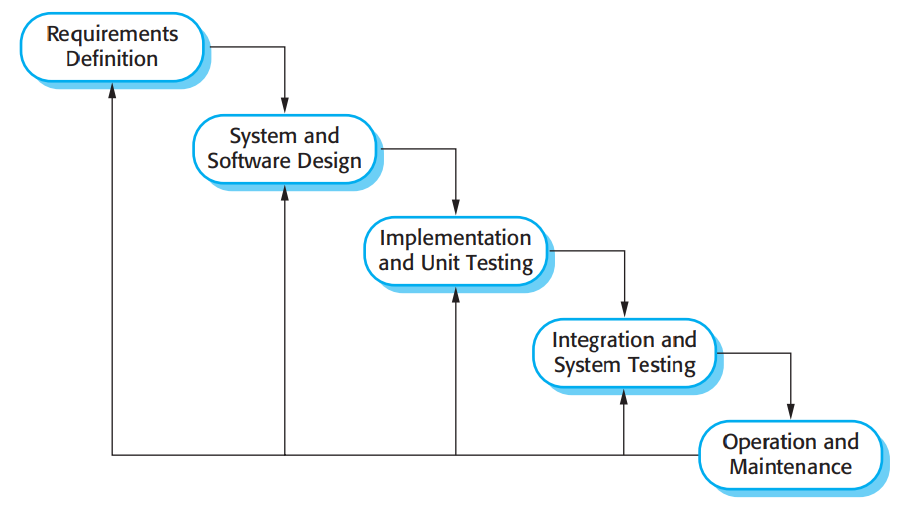
\includegraphics[width=0.7\linewidth]{images/modello-a-cascata.PNG}
    \caption{Il modello a cascata}
    \label{fig:modello-a-cascata}
\end{figure}

Le fasi del modello a cascata riflettono direttamente le attività fondamentali dello sviluppo software:
\begin{enumerate}
    \item Analisi e definizione dei requisiti.
    \item Progettazione di sistema e software.
    \item Implementazione e test unitari.
    \item Integrazione e test di sistema.
    \item Operazione e manutenzione.
\end{enumerate}
In linea di principio, il risultato di ciascuna fase del modello a cascata è uno o più documenti approvati ("firmati"). La fase successiva non dovrebbe iniziare finché la fase precedente non è completata. 

La suddivisione rigida del progetto in fasi distinte rende difficile rispondere ai cambiamenti nei requisiti del cliente. Pertanto, questo modello è appropriato solo quando i requisiti sono ben compresi e i cambiamenti saranno piuttosto limitati durante il processo di progettazione.
Pochi sistemi aziendali hanno requisiti stabili. 

Il modello a cascata è utilizzato principalmente per grandi progetti di ingegneria dei sistemi in cui un sistema viene sviluppato in più siti. In queste circostanze, la natura pianificata del modello a cascata aiuta a coordinare il lavoro.

\subsection{Sviluppo incrementale}
Lo sviluppo incrementale si basa sull'idea di sviluppare un'implementazione iniziale, ottenere feedback dagli utenti e da altri, e far evolvere il software attraverso diverse versioni fino a quando non è stato sviluppato il sistema richiesto (Figura \ref{fig:incremental-development}). 

\begin{figure}[ht]
    \centering
    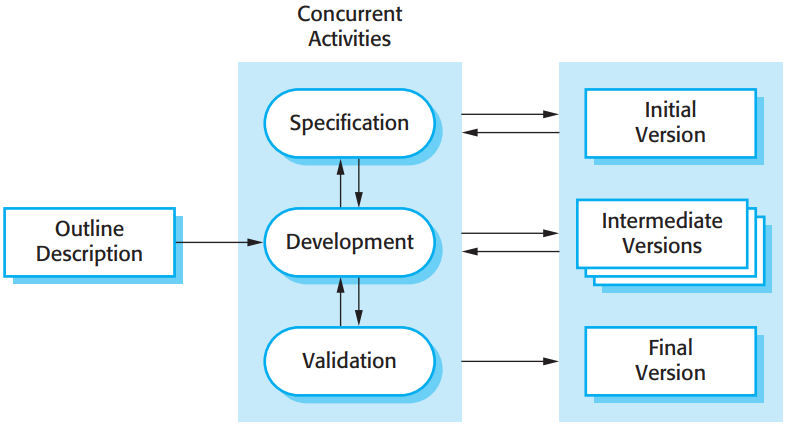
\includegraphics[width=0.6\linewidth]{images/incremental-development.PNG}
    \caption{Sviluppo incrementale}
    \label{fig:incremental-development}
\end{figure}

Lo sviluppo incrementale presenta tre importanti vantaggi rispetto al modello a cascata:
\begin{enumerate}
    \item \textit{Riduzione dei costi per le modifiche ai requisiti:} L'ammontare di analisi e documentazione che deve essere rifatta è significativamente inferiore rispetto a quanto richiesto dal modello a cascata.
    \item \textit{Facilità di ottenere feedback dai clienti:} I clienti possono commentare le dimostrazioni del software e vedere quanto è stato implementato.
    \item \textit{Consegna e distribuzione precoce di software utile:} I clienti possono utilizzare e trarre valore dal software prima rispetto a quanto possibile con un processo a cascata.
\end{enumerate}
Da una prospettiva gestionale, l'approccio incrementale presenta due problemi:
\begin{enumerate}
    \item \textit{Il processo non è visibile:} I manager hanno bisogno di risultati regolari per misurare i progressi. Se i sistemi vengono sviluppati rapidamente, non è economicamente efficace produrre documenti che riflettano ogni versione del sistema.
    \item \textit{La struttura del sistema tende a degradare:} I cambiamenti regolari portano a codice disordinato mentre vengono aggiunte nuove funzionalità in qualsiasi modo possibile. Diventa sempre più difficile e costoso aggiungere nuove caratteristiche a un sistema.
\end{enumerate}

\subsection{Integrazione e configurazione}
Nella maggior parte dei progetti software, c'è un certo riutilizzo del software. Questo riutilizzo informale avviene indipendentemente dal processo di sviluppo utilizzato. Gli approcci orientati al riutilizzo si basano su un insieme di componenti software riutilizzabili e su un framework di integrazione per la composizione di questi componenti.

Tre tipi di componenti software sono frequentemente riutilizzati:
\begin{enumerate}
    \item Sistemi applicativi stand-alone che sono configurati per l'uso in un ambiente particolare.
    \item Collezioni di oggetti sviluppate come componente o come pacchetto da integrare con un framework di componenti, come il framework Java Spring (Wheeler e White 2013).
    \item Web services che sono sviluppati secondo standard di servizio e che sono disponibili per l'invocazione remota su Internet.
\end{enumerate}
La Figura \ref{fig:reuse-oriented-software-engineering} mostra un modello di processo generale per lo sviluppo basato sul riutilizzo, incentrato su integrazione e configurazione. 

\begin{figure}[ht]
    \centering
    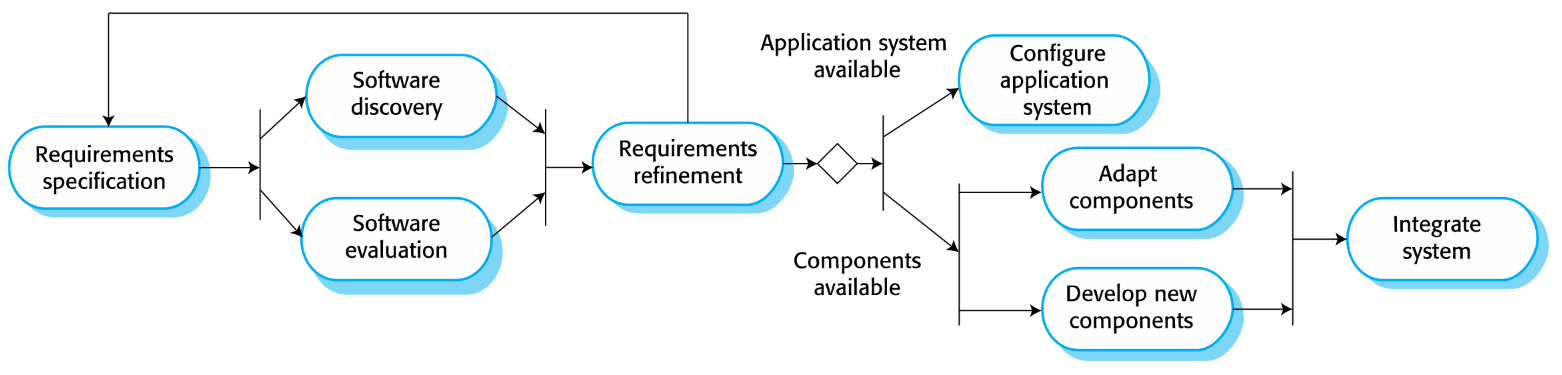
\includegraphics[width=\linewidth]{images/reuse-oriented-software-engineering.PNG}
    \caption{Ingegneria del software orientata al riutilizzo}
    \label{fig:reuse-oriented-software-engineering}
\end{figure}

Le fasi di questo processo sono:
\begin{enumerate}
    \item Specificazione dei requisiti.
    \item Scoperta e valutazione del software.
    \item Raffinamento dei requisiti.
    \item Configurazione del sistema applicativo.
    \item Adattamento e integrazione dei componenti.
\end{enumerate}

L'ingegneria del software orientata al riutilizzo, basata su configurazione e integrazione, ha il vantaggio evidente di ridurre la quantità di software da sviluppare, riducendo così costi e rischi. Di solito porta anche a una consegna più rapida del software. Tuttavia, i compromessi sui requisiti sono inevitabili, e questo può portare a un sistema che non soddisfa le reali esigenze degli utenti. Inoltre, si perde parte del controllo sull'evoluzione del sistema poiché le nuove versioni dei componenti riutilizzabili non sono sotto il controllo dell'organizzazione che li utilizza.

\section{Attività di processo}
I veri processi software sono sequenze intrecciate di attività tecniche, collaborative e manageriali, con l'obiettivo complessivo di specificare, progettare, implementare e testare un sistema software.

Le quattro attività di processo di base di specifica, sviluppo, convalida ed evoluzione sono organizzate in modo diverso nei diversi processi di sviluppo. Nel modello waterfall, sono organizzate in sequenza, mentre nello sviluppo incrementale sono intrecciate.

\subsection{Specificazione del software}
La specificazione del software, o ingegneria dei requisiti, è il processo di comprensione e definizione dei servizi richiesti dal sistema e identificazione delle limitazioni sul funzionamento e sullo sviluppo del sistema.

Il processo di ingegneria dei requisiti (Figura \ref{fig:requirements-engineering-process}) ha lo scopo di produrre un documento di requisiti concordato che specifichi un sistema in grado di soddisfare le esigenze degli stakeholder.

\begin{figure}[ht]
    \centering
    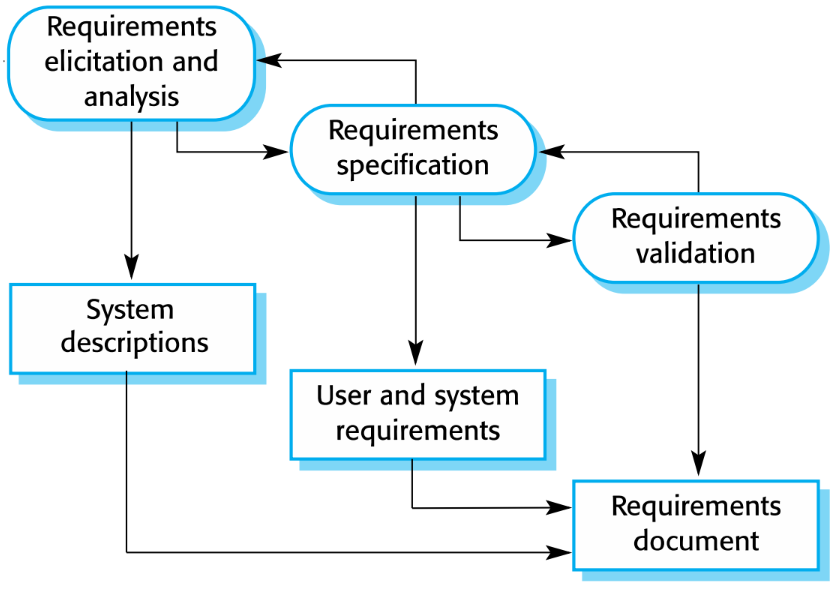
\includegraphics[width=0.5\linewidth]{images/requirements-engineering-process.PNG}
    \caption{Il processo di ingegneria dei requisiti}
    \label{fig:requirements-engineering-process}
\end{figure}

Ci sono tre attività principali nel processo di ingegneria dei requisiti:
\begin{enumerate}
    \item \textit{Elicitazione e analisi dei requisiti:} Questo è il processo di derivazione dei requisiti del sistema attraverso l'osservazione dei sistemi esistenti, discussioni con potenziali utenti e acquirenti, analisi dei compiti, e così via.
    \item \textit{Specificazione dei requisiti:} La specificazione dei requisiti è l'attività di tradurre le informazioni raccolte durante l'analisi dei requisiti in un documento che definisce un insieme di requisiti.
    \item \textit{Validazione dei requisiti:} Questa attività verifica i requisiti per realismo, coerenza e completezza.
\end{enumerate}

\subsection{Progettazione e implementazione del software}
La fase di implementazione dello sviluppo software è il processo di sviluppo di un sistema eseguibile da consegnare al cliente. A volte ciò comporta attività separate di progettazione software e programmazione. Tuttavia, se viene utilizzato un approccio agile allo sviluppo, progettazione e implementazione sono intrecciate.

Un design software è una descrizione della struttura del software da implementare, dei modelli e delle strutture dei dati utilizzati dal sistema, delle interfacce tra i componenti del sistema e, a volte, degli algoritmi utilizzati.

La Figura \ref{fig:general-model-desing-process} è un modello astratto del processo di design che mostra gli input al processo di design, le attività del processo e le uscite del processo.

\begin{figure}[ht]
    \centering
    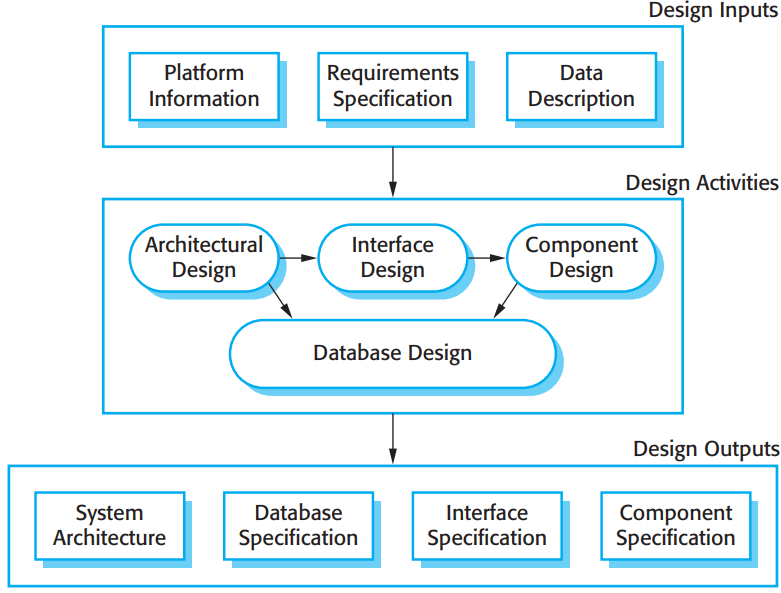
\includegraphics[width=0.6\linewidth]{images/general-model-desing-process.PNG}
    \caption{Un modello generale del processo di progettazione}
    \label{fig:general-model-desing-process}
\end{figure}

La Figura \ref{fig:general-model-desing-process} mostra quattro attività che possono far parte del processo di design per sistemi informativi:
\begin{enumerate}
    \item \textit{Design architetturale:} identificare la struttura complessiva del sistema, i componenti principali (a volte chiamati sottosistemi o moduli), le loro relazioni e come sono distribuiti.
    \item \textit{Design del database:} progettare le strutture dei dati del sistema e come queste devono essere rappresentate in un database.
    \item \textit{Design dell'interfaccia:} definire le interfacce tra i componenti del sistema.
    \item \textit{Selezione e design dei componenti:} cercare componenti riutilizzabili e, se non sono disponibili componenti adatti, progettare nuovi componenti software.
\end{enumerate}
Lo sviluppo di un programma per implementare un sistema segue naturalmente dalla progettazione del sistema. Il software viene implementato sviluppando uno o più programmi o configurando un sistema applicativo. Progettazione e implementazione sono attività intervallate per la maggior parte dei tipi di sistema software. La programmazione è un'attività individuale, e non esiste un processo generale che viene solitamente seguito. Normalmente, i programmatori effettuano alcuni test del codice che hanno sviluppato. Questo spesso rivela difetti del programma (bug) che devono essere rimossi dal programma. Trovare e correggere i difetti del programma è chiamato debugging.

\subsection{Validazione del software}
La validazione del software o, più in generale, verifica e validazione (V\&V), ha lo scopo di dimostrare che un sistema sia conforme alla sua specifica e soddisfi le aspettative del cliente del sistema. Il testing del programma, in cui il sistema viene eseguito utilizzando dati di test simulati, è la principale tecnica di validazione. La validazione può anche comportare il controllo dei processi, come ispezioni e revisioni, in ogni fase del processo software, dalla definizione dei requisiti degli utenti allo sviluppo del programma. Tuttavia, la maggior parte del tempo e dell’impegno dedicati alla V\&V è spesa nel testing del programma.

La Figura \ref{fig:stages-of-testing} mostra un processo di testing in tre fasi in cui i componenti del sistema vengono testati individualmente e poi il sistema integrato viene testato.

\begin{figure}[ht]
    \centering
    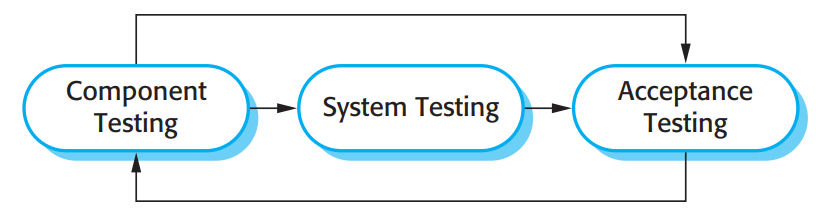
\includegraphics[width=0.5\linewidth]{images/stages-of-testing.PNG}
    \caption{Fasi di test}
    \label{fig:stages-of-testing}
\end{figure}

Le fasi del processo di testing sono:
\begin{enumerate}
    \item \textit{Testing dei componenti:} ogni componente viene testato indipendentemente. I componenti possono essere entità semplici come funzioni o classi di oggetti, o possono essere raggruppamenti coerenti di queste entità.
    \item \textit{Testing del sistema:} questo processo si concentra sulla ricerca di errori che derivano da interazioni inaspettate tra i componenti e problemi con le interfacce dei componenti. Si occupa anche di dimostrare che il sistema soddisfi i requisiti funzionali e non funzionali, e di testare le proprietà emergenti del sistema.
    \item \textit{Testing da parte del cliente:} il sistema viene testato dal cliente del sistema (o da un cliente potenziale) piuttosto che con dati di test simulati. Il testing da parte del cliente può anche rivelare problemi relativi ai requisiti, dove le funzionalità del sistema non soddisfano realmente le esigenze degli utenti o le prestazioni del sistema sono inaccettabili.
\end{enumerate}
Quando viene utilizzato un processo di plan-driven, il testing è guidato da un insieme di piani di test. Un team di tester indipendente lavora a partire da questi piani di test, che sono stati sviluppati dalla specifica e dal design del sistema. La Figura \ref{fig:testing-phases-plan-driven-software} illustra come i piani di test siano il collegamento tra le attività di testing e di sviluppo. Questo è talvolta chiamato il modello a V dello sviluppo (ruotalo di lato per vedere la V). Il modello a V mostra le attività di validazione del software che corrispondono a ciascuna fase del modello di processo a cascata.

\begin{figure}[ht]
    \centering
    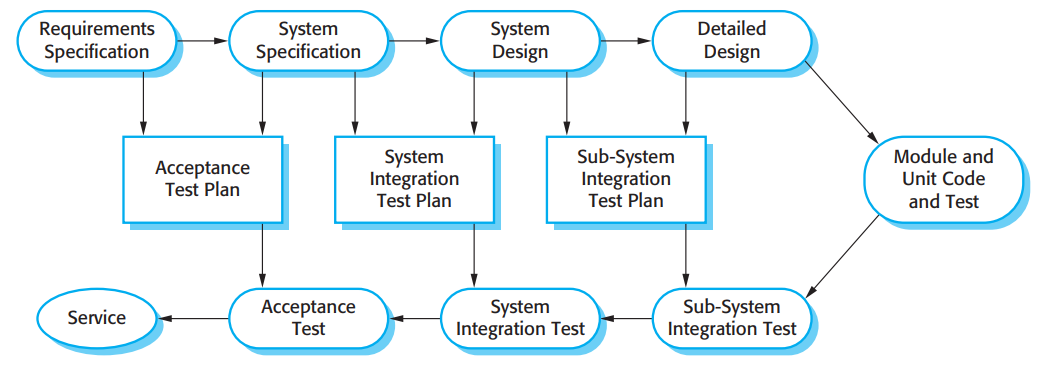
\includegraphics[width=0.9\linewidth]{images/testing-phases-plan-driven-software.PNG}
    \caption{Fasi di test in un processo software plan-driven}
    \label{fig:testing-phases-plan-driven-software}
\end{figure}

\subsection{Evoluzione del software}
La flessibilità del software è una delle principali ragioni per cui sempre più software viene incorporato in sistemi complessi e di grandi dimensioni. Modifiche al software possono essere effettuate in qualsiasi momento durante o dopo lo sviluppo del sistema.

Pochissimi sistemi software sono completamente nuovi; è quindi molto più sensato vedere lo sviluppo e la manutenzione come un continuum. Piuttosto che considerare due processi separati, è più realistico pensare all'ingegneria del software come a un processo evolutivo (Figura \ref{fig:system-evoluzion}), in cui il software viene continuamente modificato nel corso della sua vita in risposta a requisiti e bisogni dei clienti in evoluzione.

\begin{figure}[ht]
    \centering
    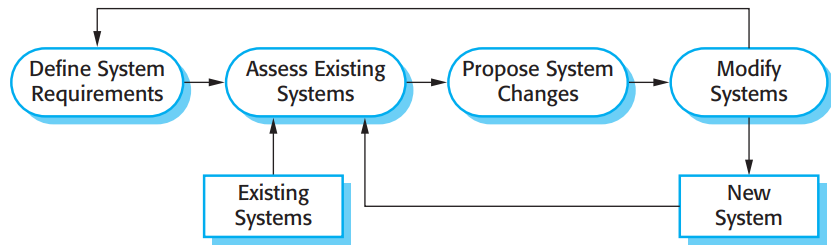
\includegraphics[width=0.6\linewidth]{images/system-evoluzion.PNG}
    \caption{Evoluzione del sistema}
    \label{fig:system-evoluzion}
\end{figure}

\section{Affrontare il cambiamento}
Il cambiamento è inevitabile in tutti i grandi progetti software. I requisiti del sistema cambiano mentre le aziende rispondono a pressioni esterne, competizione e cambiamenti nelle priorità di gestione. Con l'emergere di nuove tecnologie, diventano possibili nuovi approcci al design e all'implementazione. Pertanto, qualunque modello di processo software venga utilizzato, è essenziale che possa accogliere i cambiamenti nel software in fase di sviluppo.

I cambiamenti aumentano i costi di sviluppo software poiché generalmente significa che il lavoro già completato deve essere rifatto. Questo è noto come rielaborazione.

Due approcci correlati possono essere utilizzati per ridurre i costi di rielaborazione:
\begin{enumerate}
    \item \textit{Anticipazione dei cambiamenti:} il processo software include attività in grado di anticipare o prevedere possibili cambiamenti prima che siano necessarie rielaborazioni significative. Ad esempio, potrebbe essere sviluppato un sistema prototipo per mostrare alcune funzionalità chiave del sistema ai clienti.
    \item \textit{Tolleranza ai cambiamenti:} il processo e il software sono progettati in modo che le modifiche possano essere apportate facilmente al sistema. Ciò comporta normalmente una forma di sviluppo incrementale. Le modifiche proposte possono essere implementate in incrementi che non sono stati ancora sviluppati. Se ciò non è possibile, solo un singolo incremento (una piccola parte del sistema) potrebbe dover essere modificato per incorporare il cambiamento.
\end{enumerate}
Vediamo due modi per affrontare il cambiamento e i requisiti del sistema in evoluzione:
\begin{enumerate}
    \item \textit{Prototipazione del sistema:} una versione del sistema o parte di essa è sviluppata rapidamente per verificare i requisiti del cliente e la fattibilità delle decisioni progettuali. Questo è un metodo di anticipazione del cambiamento.
    \item \textit{Consegna incrementale:} gli incrementi del sistema vengono consegnati al cliente per commenti e sperimentazione. Questo supporta sia l'evitamento del cambiamento sia la tolleranza ai cambiamenti.
\end{enumerate}

\subsection{Prototipazione}
Un prototipo è una versione preliminare di un sistema software utilizzata per dimostrare concetti, provare opzioni di design e approfondire la comprensione del problema e delle possibili soluzioni.

Un prototipo software può essere utilizzato in un processo di sviluppo software per aiutare a prevedere i cambiamenti che potrebbero essere necessari:
\begin{enumerate}
    \item Nel processo di ingegneria dei requisiti, un prototipo può aiutare con l'estrazione e la validazione dei requisiti del sistema.
    \item Nel processo di design del sistema, un prototipo può essere utilizzato per esplorare soluzioni software e nello sviluppo di un'interfaccia utente per il sistema.
\end{enumerate}
I prototipi di sistema consentono agli utenti potenziali di vedere quanto bene il sistema supporti il loro lavoro. Possono generare nuove idee per requisiti e identificare aree di forza e debolezza nel software. Possono quindi proporre nuovi requisiti di sistema. Inoltre, man mano che il prototipo viene sviluppato, possono emergere errori e omissioni nei requisiti del sistema.

Un modello di processo per lo sviluppo di prototipi è mostrato nella Figura \ref{fig:process-prototype}. Gli obiettivi della prototipazione dovrebbero essere esplicitati fin dall'inizio del processo.

\begin{figure}[ht]
    \centering
    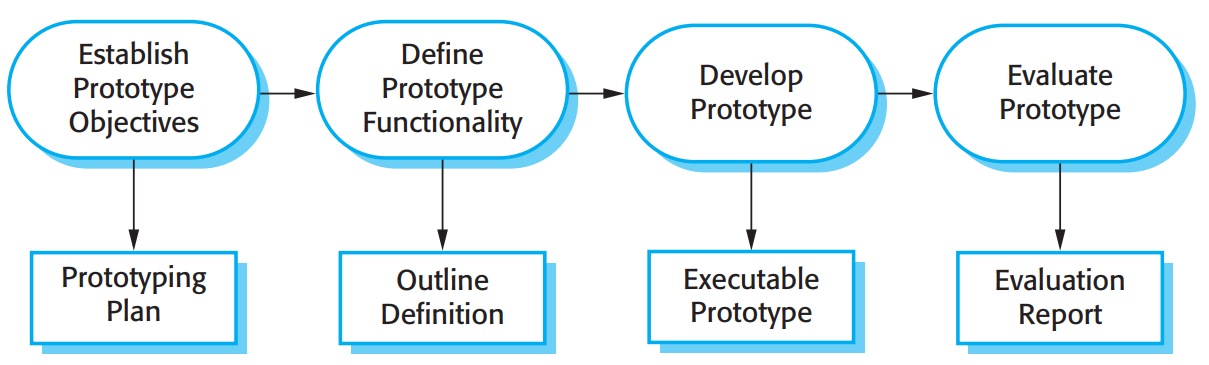
\includegraphics[width=0.6\linewidth]{images/process-prototype.PNG}
    \caption{Il processo di sviluppo del prototipo}
    \label{fig:process-prototype}
\end{figure}

La fase successiva del processo è decidere cosa includere e, forse più importante, cosa escludere dal sistema prototipo. Per ridurre i costi di prototipazione e accelerare il programma di consegna, si può decidere di escludere alcune funzionalità dal prototipo. Il prototipo dovrebbe concentrarsi su aree del prodotto che non sono ben comprese e il controllo degli errori e il ripristino potrebbero non essere inclusi nel prototipo.
L'ultima fase del processo è la valutazione del prototipo.

I prototipi dovrebbero essere scartati dopo lo sviluppo poiché non sono una buona base per un sistema di produzione. Infatti: potrebbe essere impossibile adattare il sistema per soddisfare i requisiti non funzionali; i prototipi sono normalmente privi di documentazione; la struttura del prototipo è solitamente degradabile a causa del cambiamento rapido; il prototipo probabilmente non soddisferà gli standard di qualità normali dell'organizzazione.

\subsection{Consegna incrementale}
La consegna incrementale (Figura \ref{fig:incremental-delivery}) è un approccio allo sviluppo software in cui alcuni degli incrementi sviluppati vengono consegnati al cliente e implementati nel loro ambiente di lavoro. In un processo di consegna incrementale, i clienti definiscono quali servizi sono più importanti e quali sono meno importanti per loro. Vengono quindi definiti diversi incrementi di consegna, ciascuno dei quali fornisce un sottoinsieme delle funzionalità del sistema.

\begin{figure}[ht]
    \centering
    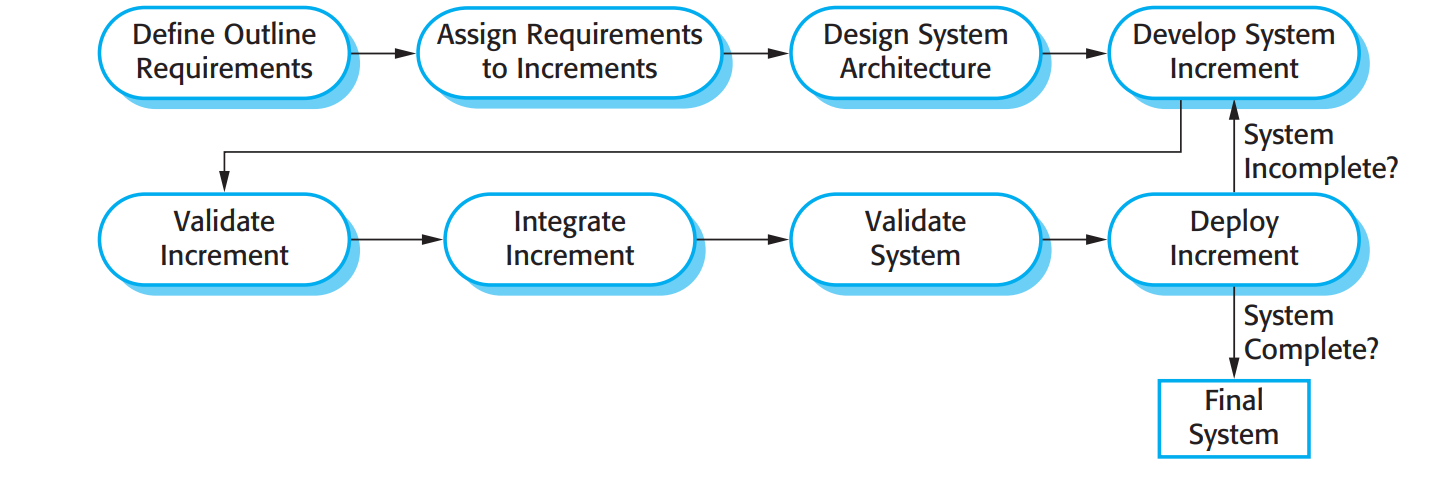
\includegraphics[width=0.7\linewidth]{images/incremental-delivery.PNG}
    \caption{Consegna incrementale}
    \label{fig:incremental-delivery}
\end{figure}

Una volta identificati gli incrementi di sistema, i requisiti per i servizi da consegnare nel primo incremento vengono definiti in dettaglio e quell'incremento viene sviluppato. Man mano che nuovi incrementi vengono completati, vengono integrati con gli incrementi esistenti in modo che la funzionalità del sistema migliori con ogni incremento consegnato.

La consegna incrementale presenta diversi vantaggi:
\begin{enumerate}
    \item I clienti possono utilizzare i primi incrementi come prototipi e acquisire esperienza che informi i loro requisiti per gli incrementi successivi del sistema.
    \item I clienti non devono aspettare fino a quando l'intero sistema è consegnato prima di poter trarre valore da esso. Il primo incremento soddisfa i loro requisiti più critici, quindi possono utilizzare il software immediatamente.
    \item Il processo mantiene i benefici dello sviluppo incrementale in quanto dovrebbe essere relativamente facile incorporare cambiamenti nel sistema.
    \item Poiché i servizi di massima priorità vengono consegnati per primi e gli incrementi successivi vengono poi integrati, i servizi di sistema più importanti ricevono il maggior numero di test.
\end{enumerate}
Tuttavia, ci sono problemi con la consegna incrementale. In pratica, funziona solo in situazioni in cui viene introdotto un sistema completamente nuovo e i valutatori del sistema hanno tempo per sperimentare con il nuovo sistema. I principali problemi con questo approccio sono:
\begin{enumerate}
    \item La maggior parte dei sistemi richiede un insieme di funzionalità di base utilizzate da diverse parti del sistema. Poiché i requisiti non sono definiti in dettaglio fino a quando non deve essere implementato un incremento, può essere difficile identificare le funzionalità comuni necessarie per tutti gli incrementi.
    \item L'essenza dei processi iterativi è che la specifica viene sviluppata in concomitanza con il software. Tuttavia, questo va in conflitto con il modello di approvvigionamento di molte organizzazioni, in cui la specifica completa del sistema fa parte del contratto di sviluppo del sistema.
\end{enumerate}

\section{Miglioramento dei processi}
Molte aziende software si sono rivolte al miglioramento dei processi software come modo per aumentare la qualità del loro software, ridurre i costi o accelerare i loro processi di sviluppo. Il miglioramento del processo significa comprendere i processi esistenti e cambiarli per aumentare la qualità del prodotto e/o ridurre i costi e i tempi di sviluppo.

Vengono utilizzati due approcci abbastanza diversi per il miglioramento e il cambiamento dei processi:
\begin{enumerate}
    \item L'\textit{approccio della maturità del processo}, che si è concentrato sul miglioramento della gestione dei processi e dei progetti e sull'introduzione di buone pratiche di ingegneria del software in un'organizzazione. Il livello di maturità del processo riflette il grado in cui sono state adottate buone pratiche tecniche e di gestione nei processi di sviluppo software dell'organizzazione.
    \item L'\textit{approccio agile}, che si è concentrato sullo sviluppo iterativo e sulla riduzione dei costi generali nel processo software. Le caratteristiche principali dei metodi agili sono la rapida consegna delle funzionalità e la reattività ai cambiamenti nei requisiti del cliente.
\end{enumerate}
Il processo generale di miglioramento del processo che sottende l'approccio della maturità del processo è un processo ciclico, come mostrato nella Figura \ref{fig:process-improvement-cycle}. 

\begin{figure}[ht]
    \centering
    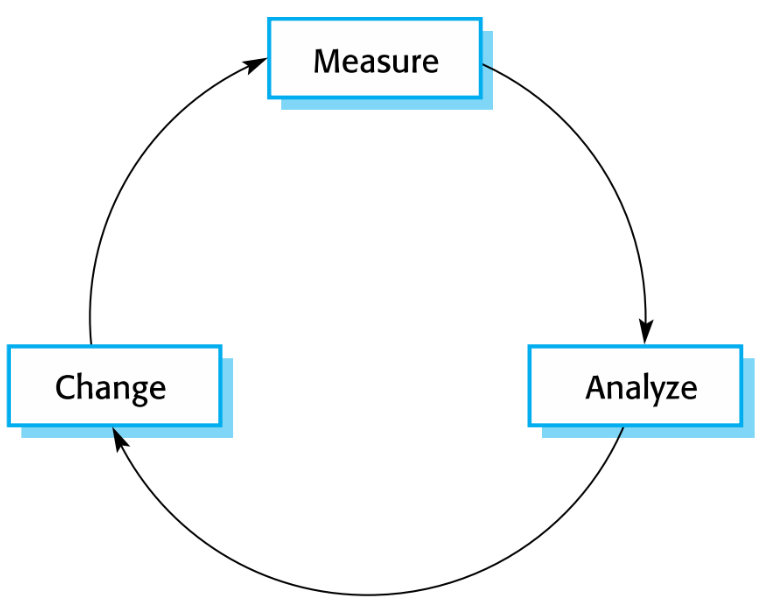
\includegraphics[width=0.4\linewidth]{images/process-improvement-cycle.PNG}
    \caption{Il ciclo di miglioramento dei processi}
    \label{fig:process-improvement-cycle}
\end{figure}

Le fasi in questo processo sono:
\begin{enumerate}
    \item \textit{Misurazione del processo:} si misura uno o più attributi del processo software o del prodotto. Queste misurazioni formano una base di riferimento che aiuta a decidere se i miglioramenti del processo sono stati efficaci.
    \item \textit{Analisi del processo:} il processo attuale viene valutato e vengono identificati punti deboli e colli di bottiglia. Durante questa fase possono essere sviluppati modelli di processo (a volte chiamati mappe di processo) che descrivono il processo.
    \item \textit{Cambiamento del processo:} vengono proposti cambiamenti al processo per affrontare alcune delle debolezze identificate. Questi vengono introdotti e il ciclo riprende per raccogliere dati sull'efficacia delle modifiche.
\end{enumerate}
Senza dati concreti su un processo o sul software sviluppato utilizzando quel processo, è impossibile valutare il valore del miglioramento del processo. Tuttavia, le aziende che avviano il processo di miglioramento potrebbero non avere dati sui processi disponibili come base di riferimento per il miglioramento. Pertanto, come parte del primo ciclo di cambiamenti, potrebbe essere necessario raccogliere dati sul processo software e misurare le caratteristiche del prodotto software.

L'idea di maturità del processo è stata introdotta alla fine degli anni '80 quando il Software Engineering Institute (SEI) propose il loro modello di maturità della capacità dei processi (Humphrey 1988). La maturità dei processi di un'azienda software riflette la gestione dei processi, la misurazione e l'uso di buone pratiche di ingegneria del software all'interno dell'azienda. Sono stati proposti cinque livelli di maturità del processo, come mostrato nella Figura \ref{fig:capability-maturity-levels}.

\begin{figure}[ht]
    \centering
    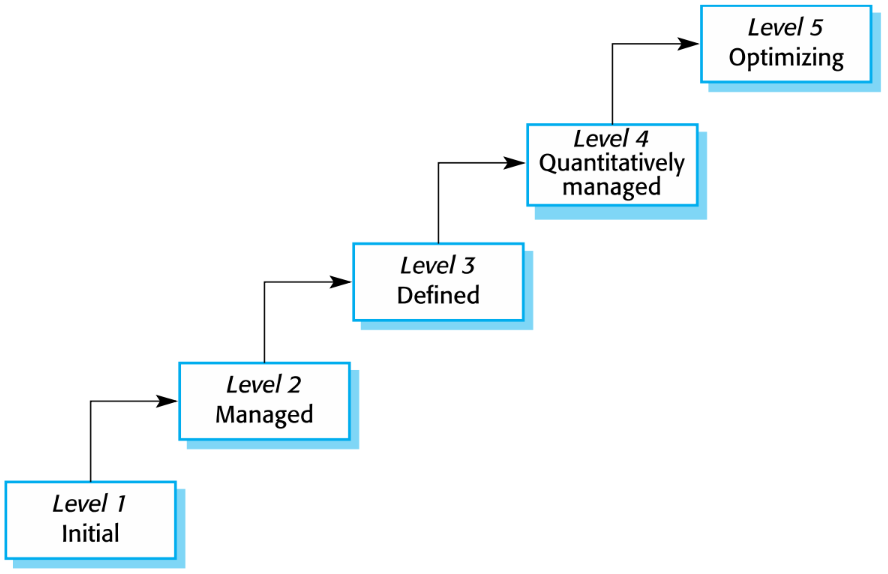
\includegraphics[width=0.6\linewidth]{images/capability-maturity-levels.PNG}
    \caption{Livelli di maturità delle capacità}
    \label{fig:capability-maturity-levels}
\end{figure}

I livelli nel modello di maturità del processo sono:
\begin{enumerate}
    \item \textit{Iniziale:} gli obiettivi associati all'area del processo sono soddisfatti e, per tutti i processi, l'ambito del lavoro da svolgere è esplicitamente definito e comunicato ai membri del team.
    \item \textit{Gestito:} a questo livello, gli obiettivi associati all'area del processo sono raggiunti e le politiche organizzative sono in atto per definire quando ciascun processo dovrebbe essere utilizzato.
    \item \textit{Definito:} questo livello si concentra sulla standardizzazione e distribuzione organizzativa dei processi.
    \item \textit{Gestito quantitativamente:} a questo livello, c'è una responsabilità organizzativa per utilizzare metodi statistici e altri metodi quantitativi per controllare i sotto-processi.
    \item \textit{Ottimizzante:} a questo livello più alto, l'organizzazione deve utilizzare le misurazioni del processo e del prodotto per guidare il miglioramento del processo.
\end{enumerate}

\newpage
\section{Punti chiave}
\begin{center}
\begin{minipage}{\textwidth}
\colorbox{lightgray}{
\parbox{\linewidth}{
\begin{itemize} 
    \item I processi software sono le attività coinvolte nella produzione di un sistema software. I modelli di processo software sono rappresentazioni astratte di questi processi.
    \item I modelli di processo generali descrivono l'organizzazione dei processi software. Esempi di questi modelli generali includono il modello a cascata, lo sviluppo incrementale e la configurazione e integrazione di componenti riutilizzabili.
    \item L'ingegneria dei requisiti è il processo di sviluppo di una specifica software.
    \item I processi di design e implementazione si occupano di trasformare una specifica dei requisiti in un sistema software eseguibile.
    \item La validazione del software è il processo di verifica che il sistema sia conforme alla sua specifica e che soddisfi le reali esigenze degli utenti del sistema.
    \item L'evoluzione del software avviene quando si modificano i sistemi software esistenti per soddisfare nuovi requisiti. I cambiamenti sono continui e il software deve evolvere per rimanere utile.
    \item I processi dovrebbero includere attività per affrontare i cambiamenti. Questo può comportare una fase di prototipazione che aiuta a evitare decisioni sbagliate sui requisiti e sul design. I processi possono essere strutturati per uno sviluppo e una consegna iterativa in modo che i cambiamenti possano essere apportati senza interrompere il sistema nel suo insieme.
    \item Le principali strategie per il miglioramento dei processi sono gli approcci agili, orientati a ridurre i costi dei processi, e gli approcci basati sulla maturità, che si fondano su una migliore gestione dei processi e sull'uso di buone pratiche di ingegneria del software.
    \item Il framework di maturità dei processi del SEI identifica livelli di maturità che corrispondono essenzialmente all'uso di buone pratiche di ingegneria del software.
\end{itemize}
}}
\end{minipage}
\end{center}